\subsection{Model Validation}

\begin{figure}[!ht]
  \caption{5-fold CV}
  \centering
    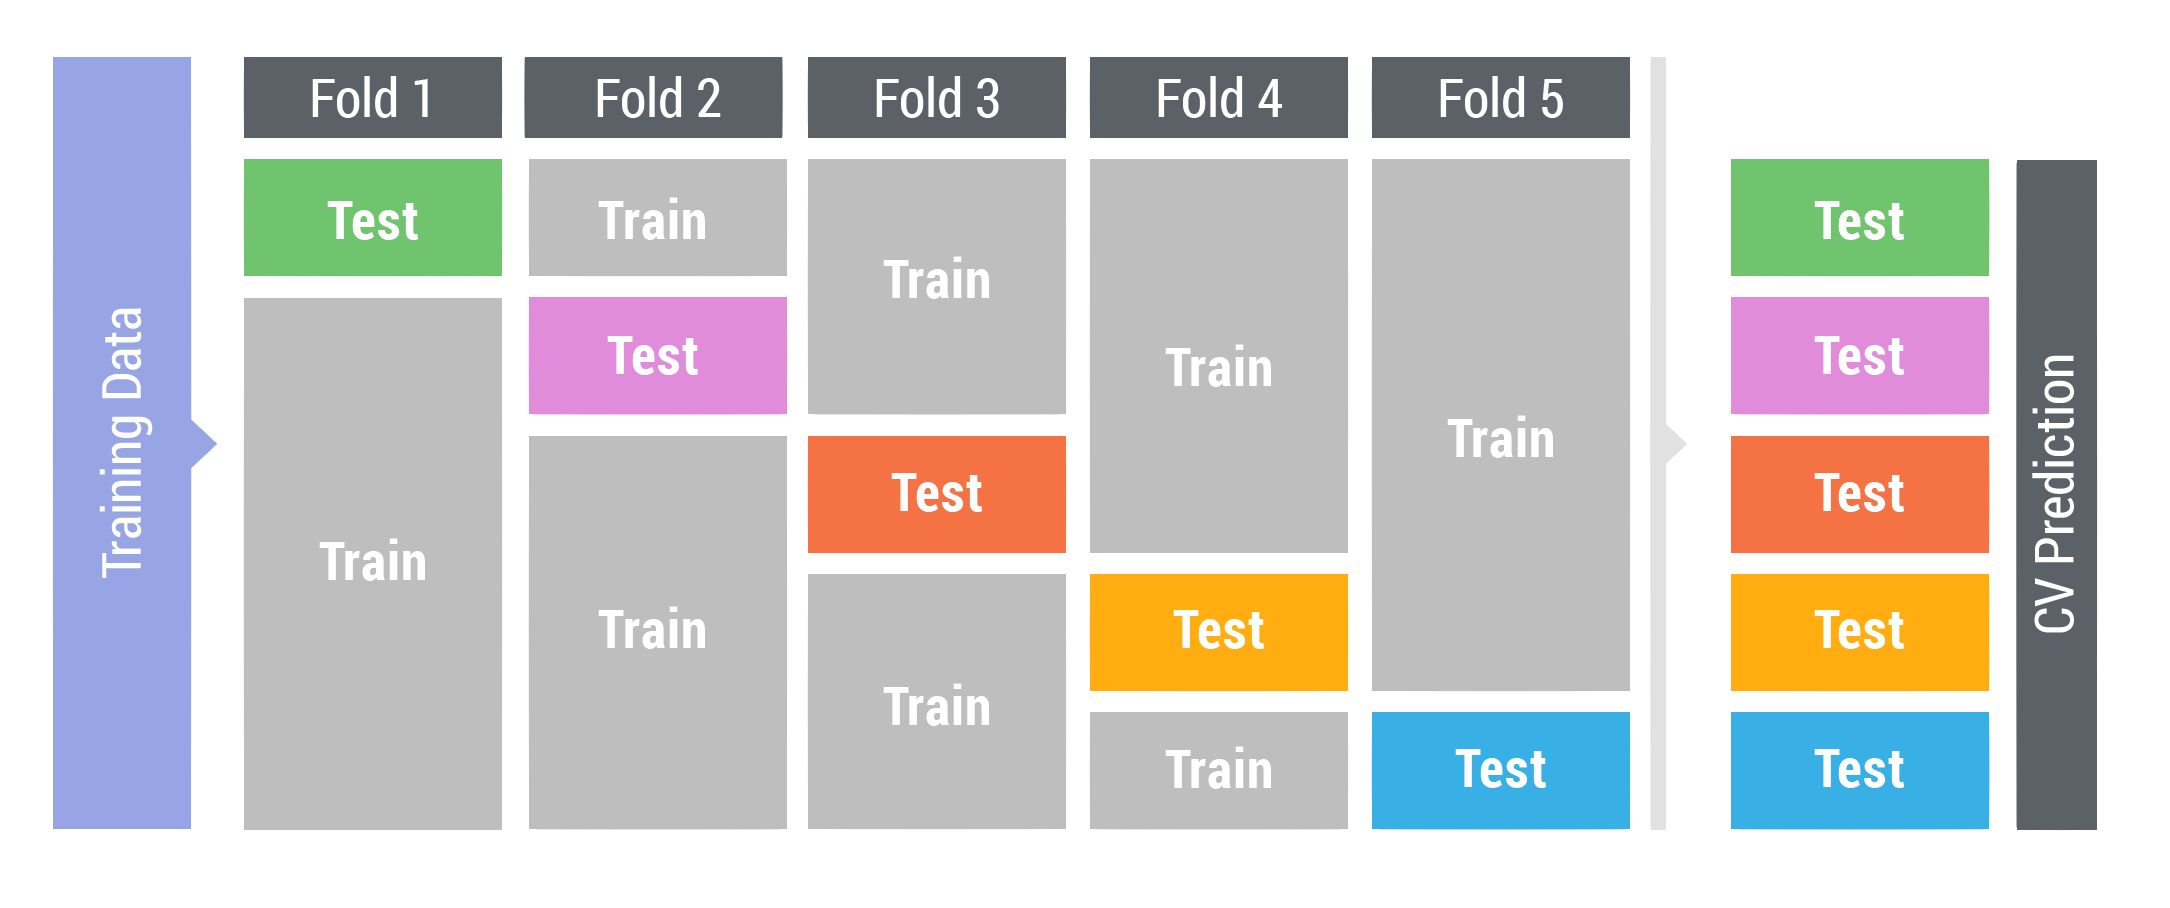
\includegraphics[width=0.5 \textwidth]{cv}
\end{figure}


We use stratified 5-fold cross validation (CV) for model validation and ensemble.
Training data are split into five folds while the sample size and dropout rate are preserved across folds.

For validation, each of single and ensemble models is trained five times. Each time, one fold is held out and the remaining four folds are used for training. Then, predictions for the hold-out folds are combined and form the model's CV prediction. CV predictions are used as inputs for ensemble model training as well as validation score calculation.

For test, each of single and ensemble models is retrained with whole training data. Then predictions for test data are used as inputs for ensemble prediction as well as for submission.
